\begin{frame}[fragile]
\frametitle{Geometry shader}
	\begin{itemize}
  \item Geometry shader is located after vertex shader (after tessellation).
	\item Geometry shader is executed per primitive - it has access to all vertices of a primitive.
	\item It can generate new geometry or modify current geometry.
  \item It can transform point into quad (usefull for particle simulation).
  \item It can be used for several effects (shadow volumes, particle systems, ...).
	\item Geometry Instancing.
	\item Transform feedback.
	\end{itemize}
\end{frame}

\begin{frame}[fragile]
\frametitle{Geometry shader - inputs/outputs}
	\begin{itemize}
	\item Type of inputs and outputs has to be specified inside geometry shader.
	{\scriptsize
	\begin{minted}[frame=lines]{glsl}
layout(points,invocations=N)in;//input primitive will be point.
//points, lines, lines_adjacency, triangles, triangles_adjacency
//geometry shader will be executed N times on each point.
	\end{minted}
	}
	\item Type of output primitive and number of output vertices has to be specified.
	{\scriptsize
	\begin{minted}[frame=lines]{glsl}
layout(triangle_strip,max_vertices=4)out;//output primitive and max number of vertices
//points, line_strip, triangle_strip
	\end{minted}
	}
	\end{itemize}
\end{frame}

\begin{frame}[fragile]
\frametitle{Geometry shader - point to quad}
	\begin{figure}[h]
		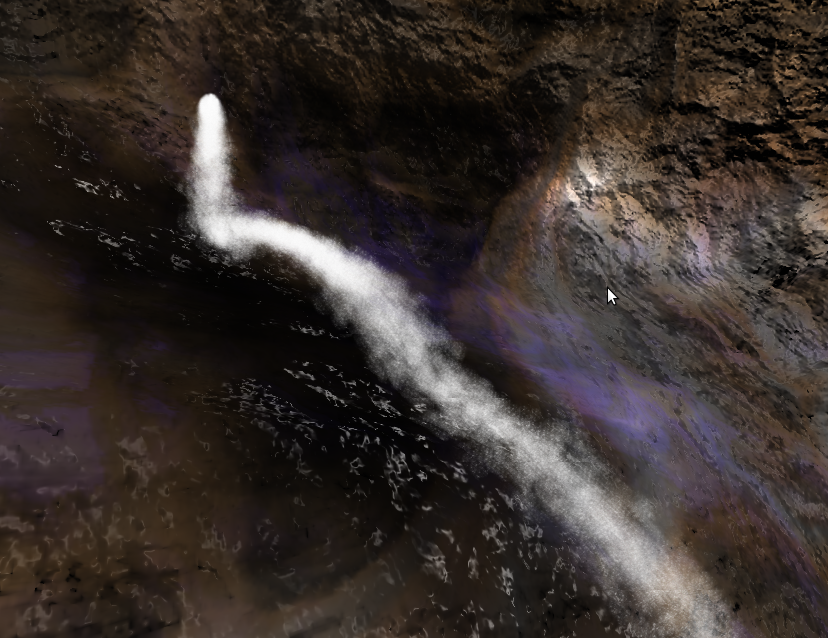
\includegraphics[width=9cm,keepaspectratio]{pics/gs.pdf}
	\end{figure}

	{\scriptsize
	\begin{minted}[frame=lines]{glsl}
#version 430

layout(points)in;
layout(triangle_strip,max_vertices=4)out;

void main(){
  gl_Position=mvp*(gl_in[0].gl_Position+vec4(-1,-1,0,0));
  EmitVertex();
  gl_Position=mvp*(gl_in[0].gl_Position+vec4(-1,+1,0,0));
  EmitVertex();
  gl_Position=mvp*(gl_in[0].gl_Position+vec4(+1,-1,0,0));
  EmitVertex();
  gl_Position=mvp*(gl_in[0].gl_Position+vec4(+1,+1,0,0));
  EmitVertex();
  EndPrimitive();
}
	\end{minted}
	}
\end{frame}

\begin{frame}[fragile]
\frametitle{Geometry shader - fullscreen quad}
	{\scriptsize
	\begin{minted}[frame=lines]{glsl}
#version 430
layout(points)in;
layout(triangle_strip,max_vertices=4)out;
void main(){
  gl_Position=vec4(-1,-1,0,1);EmitVertex();
  gl_Position=vec4(-1,+1,0,1);EmitVertex();
  gl_Position=vec4(+1,-1,0,1);EmitVertex();
  gl_Position=vec4(+1,+1,0,1);EmitVertex();
  EndPrimitive();
}
	\end{minted}
	}
	{\scriptsize
	\begin{minted}[frame=lines]{c++}
glGenVertexArrays(1,&emptyVAO);
//...
glBindVertexArray(emptyVAO);//activate VAO
glDrawArrays(GL_POINTS,0,1);
glBindVertexArray(0);//deactivate VAO
	\end{minted}
	}
\end{frame}

\begin{frame}[fragile]
\frametitle{Shadow volumes - zfail}
  \begin{figure}[h]
    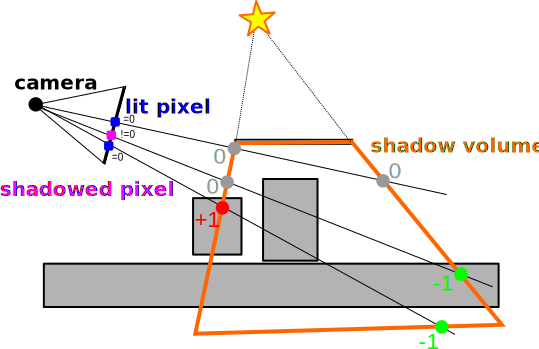
\includegraphics[width=11cm,keepaspectratio]{pics/shadowvolume.pdf}
  \end{figure}
\end{frame}

\begin{frame}[fragile]
\frametitle{Geometry shader - Shadow volumes}
  \begin{columns}[T]
    \begin{column}{.44\textwidth}
	    {\tiny
      	\begin{minted}[frame=lines]{glsl}
#version 330
layout(triangles)in;
layout(triangle_strip,max_vertices=10)out;
uniform mat4 MVP,M;//matrices
uniform vec4 LightPosition;//light position
void main(){
  vec4 LP=M*LightPosition;
  vec4 p[6];
  p[0]=gl_in[0].gl_Position;//triangle vertices
  p[1]=gl_in[1].gl_Position;
  p[2]=gl_in[2].gl_Position;
  p[3]=vec4(gl_in[0].gl_Position.xyz*LP.w-LP.xyz,0);//triangle points projected to infinity
  p[4]=vec4(gl_in[1].gl_Position.xyz*LP.w-LP.xyz,0);
  p[5]=vec4(gl_in[2].gl_Position.xyz*LP.w-LP.xyz,0);
  vec3 N=normalize(cross((p[1]-p[0]).xyz,(p[2]-p[0]).xyz));
  float Distance=dot(N,LP.xyz)-dot(N,p[0].xyz);
  if(Distance<=0){//flip volume inside out
    vec4 c=p[0];p[0]=p[1];p[1]=c;
    c=p[3];p[3]=p[4];p[4]=c;
  }
  gl_Position=MVP*p[0];EmitVertex();
  gl_Position=MVP*p[1];EmitVertex();
  gl_Position=MVP*p[3];EmitVertex();
  gl_Position=MVP*p[4];EmitVertex();
  gl_Position=MVP*p[5];EmitVertex();
  gl_Position=MVP*p[1];EmitVertex();
  gl_Position=MVP*p[2];EmitVertex();
  gl_Position=MVP*p[0];EmitVertex();
  gl_Position=MVP*p[5];EmitVertex();
  gl_Position=MVP*p[3];EmitVertex();
  EndPrimitive();
}
    	\end{minted}
   	}
    \end{column}
    \begin{column}{.48\textwidth}
	    \begin{figure}[h]
    		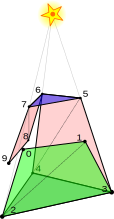
\includegraphics[width=3cm,keepaspectratio]{pics/PerTriangle.pdf}
    	\end{figure}
    \end{column}
  \end{columns}

\end{frame}

